\chapter{Tổng quan lý thuyết}
\label{Chapter2}

\section{Optical Character Recognition (OCR)}
Đầu tiên, chúng tôi xin được giới thiệu khái quát về định nghĩa về OCR \cite{impedovo1991optical}. OCR hay Optical Character Recognition (dịch là Nhận dạng ký tự quang học) là một công nghệ phát triển
mạnh mẽ, được sử dụng phổ biến thời gian gần đây. Được biết đến như một kỹ thuật scan
dữ liệu chữ viết trên hình ảnh bất kỳ, OCR giúp phát hiện và phân tích vùng văn bản xuất
hiện xung quanh ta, có thể là sách vở, biển báo,… và chuyển nó thành những ký tự số có
thể thao tác được trên máy tính hoặc các thiết bị điện tử.

Từ đó, ta có thể thực hiện những tác vụ như dịch văn bản, tự động bổ sung phần văn bản bị
khiếm khuyết hoặc dùng nó làm đầu vào của những ứng dụng cao cấp hơn (tìm kiếm, xử
lý,…). Từ những lợi ích phía trên mà hệ thống OCR mang lại, ta có thể tiết kiệm được rất
nhiều thời gian, cập nhật được thông tin nhanh và chính xác cũng như những đối tượng
như người khiếm thị có thể được hỗ trợ nhiều hơn (OCR có khả năng quét và đọc các đoạn
văn bản được đưa ra cải thiện khả năng nhận biết xung quanh của họ).

\begin{figure}
\centering
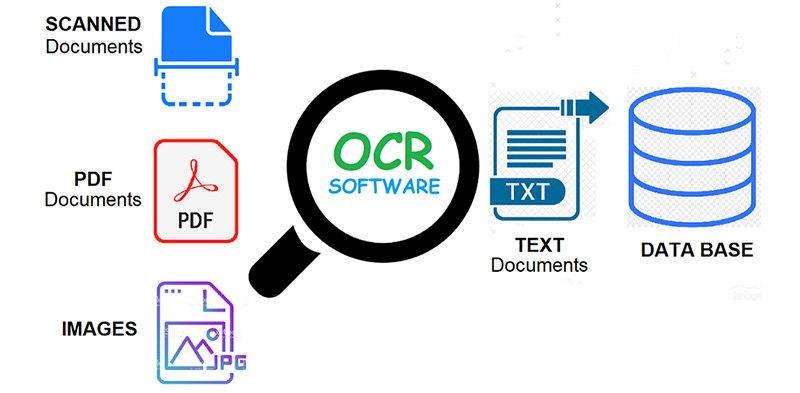
\includegraphics[width=0.9\textwidth]{mep_img/ocr-1.jpg}
\caption{OCR mang lại nhiều lợi ích cho cuộc sống \cite{ocr_intro}. }\label{fig_2.1}
\end{figure}

Tuy nhiên bên cạnh những lợi ích to lớn mà OCR mang lại, vẫn còn nhiều hạn chế mà các
mô hình OCR gặp phải:

\begin{itemize}
    \item Độ chính xác của những hệ thống này chưa cao chỉ đạt khoảng 70-80$\%$.
    \item Thời gian hoạt động với hiệu suất của mô hình chưa thật sự tương xứng. Những mô
hình chính xác cao thường có thời gian chạy lâu hơn những mô hình chính xác thấp
rất nhiều.
\item Đa dạng ngôn ngữ thực sự là một rào cản to lớn khi mà ngày càng nhiều đất nước
phát triển. Đi kèm với nó là nhu cầu cần tìm hiểu ngôn ngữ mới của người dùng sẽ ngày một tăng.
\end{itemize}

\begin{figure}
\centering
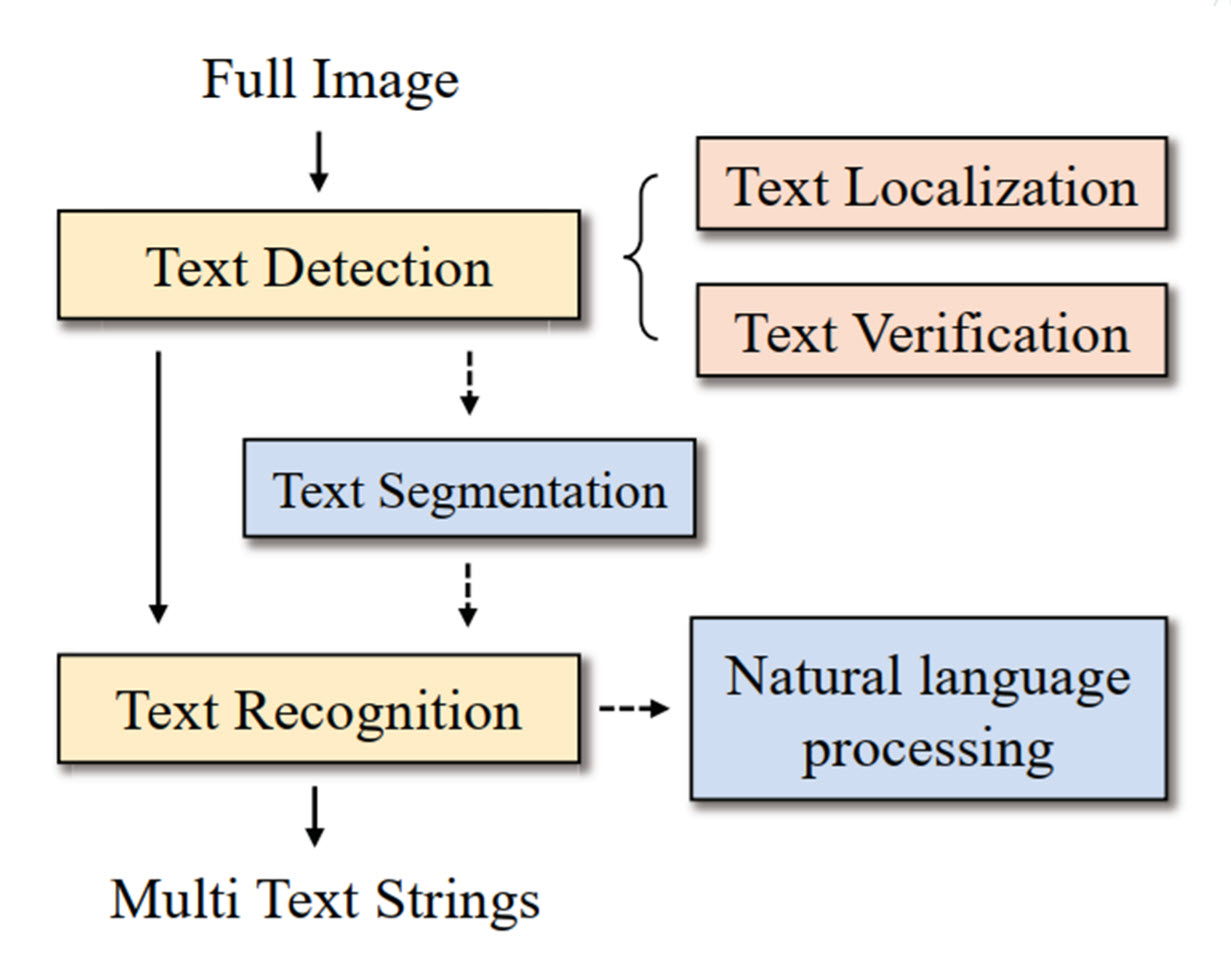
\includegraphics[width=0.9\textwidth]{mep_img/typeofproblem.jpg}
\caption{Mô hình của một số hệ thống OCR phổ biến hiện nay \cite{ocr_struct}. }\label{fig_2.2}
\end{figure}

Bên cạnh đó còn có rất nhiều lý do khác ảnh hưởng đến kết quả của bài toán OCR như:
font chữ, mật độ văn bản, ảnh nền, cấu trúc, vị trí, độ rõ nét của ảnh,...

Việt Nam là một trong những đất nước có nền kinh tế cũng như du lịch ngày một phát triển.
Nhu cầu về một hệ thống có thể nhận dạng được ngôn ngữ Việt nhưng vẫn đảm bảo về thời
gian và độ chính xác được đặt ra, giữa vô vàn hệ thống OCR có sẵn hiện nay. Trong khóa
luận này chúng tôi cũng sẽ tìm hiểu và cài đặt một mô hình nhận dạng văn bản tiếng Việt - một trong
những công đoạn quan trọng không thể thiếu của mô hình của chúng tôi. Trước tiên, ta cùng
đi tìm hiểu từng thành phần chính của một số mô hình OCR phổ biến hiện nay.



Theo như hình ~\ref{fig_2.2}, một mô hình OCR hiện nay có thể chứa nhiều công đoạn khác nhau như bản địa hóa, khai
thác đặc trưng, phát hiện văn bản và nhận dạng. Nhưng tổng quát, ta sẽ chỉ có ba công
đoạn chính là Text Detection, Text Recognition và Post-OCR.

\subsection{Text Detection}
Nhiệm vụ đầu tiên của một mô hình OCR cơ bản chính là Text Detection. Đây là quá trình
mô hình thực hiện công việc phát hiện vùng văn bản được chứa bởi hình ảnh đầu vào. Đầu
vào của công đoạn này là một hình ảnh bất kỳ và kết quả trả về chính là tọa độ của tập hợp
những bounding box (một ô hình chữ nhật chứa trọn vùng văn bản) của hình ảnh ban đầu.
Có rất nhiều phương pháp có thể được sử dụng để giải quyết bài toán text detection. Có thể
kể đến một số phương pháp truyền thống dựa vào việc xác định các vùng màu sắc, các
vùng chứa biên cạnh có trên ảnh. Các phương pháp này chủ yếu thường dựa vào một số
đặc điểm như màu sắc, hình dạng, kích thước,... của văn bản trên ảnh để có thể tìm kiếm
và trả về vị trí của chúng. Mặc dù những phương pháp kể trên thường có thể dễ dàng áp
dụng lên ảnh với thời gian ngắn trước khi trả về kết quả tuy nhiên độ chính xác của chúng
thì chưa cao.

\begin{figure}
\centering
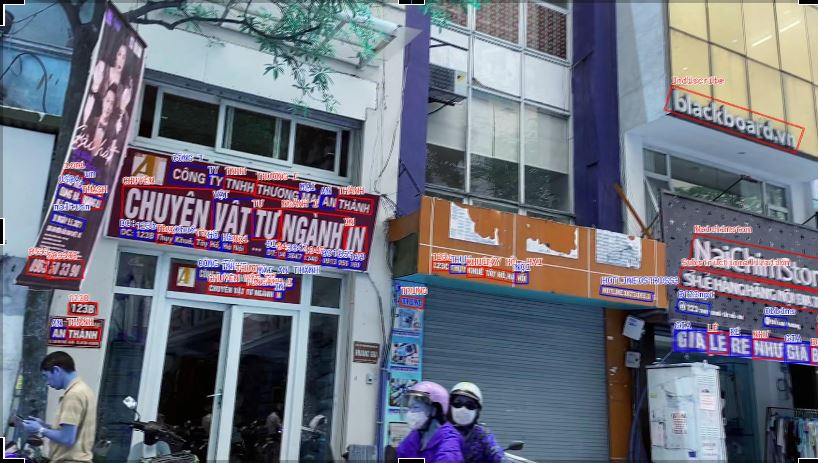
\includegraphics[width=0.9\textwidth]{mep_img/Capture.JPG}
\caption{Số lượng văn bản, nền ảnh và cấu trúc văn bản chính là những khó khăn thường gặp của một mô hình OCR.}\label{fig_2.3}
\end{figure}

Như hình ~\ref{fig_2.3}, nền của ảnh và số lượng văn bản có trong ảnh trở thành một trở ngại vô
cùng lớn trong việc đi tìm những đặc điểm, đặc trưng của văn bản trên ảnh, khiến cho độ
chính xác của những mô hình truyền thống này giảm đi khá đáng kể.
Với sự phát triển của Deep Learning trong những năm gần đây, vô vàn những mô hình Deep
Learning được sinh ra để giải quyết được bài toán text detection trong khoảng thời gian ngắn
nhưng vẫn giữ được độ chính xác cao. Một số hướng giải quyết bài toán text detection
được sử dụng trong thời gian gần đây:
\begin{itemize}
    \item Phát hiện vật thể: Ta có thể coi bài toán phát hiện văn bản là một bài toán phát hiện
vật thể (minh họa hình ~\ref{fig_2.4}), những văn bản có trong ảnh sẽ được định nghĩa và gán nhãn như một vật
thể. Một số mô hình phát hiện vật thể có thể được ứng dụng vào những phương
pháp này như CNNs \cite{delakis2008text}, VGG16 \cite{he2020realtime}, YoLo \cite{haifeng2020natural},... đặc biệt hơn là những mô hình
được sinh ra dựa vào phương pháp này để tập trung hoàn toàn vào nhiệm vụ phát
hiện văn bản như TextFuseNet (ResNeXt-101) \cite{ye2020textfusenet}, EAST \cite{zhou2017east}, CTPN \cite{tian2016detecting},…

\begin{figure}
\centering
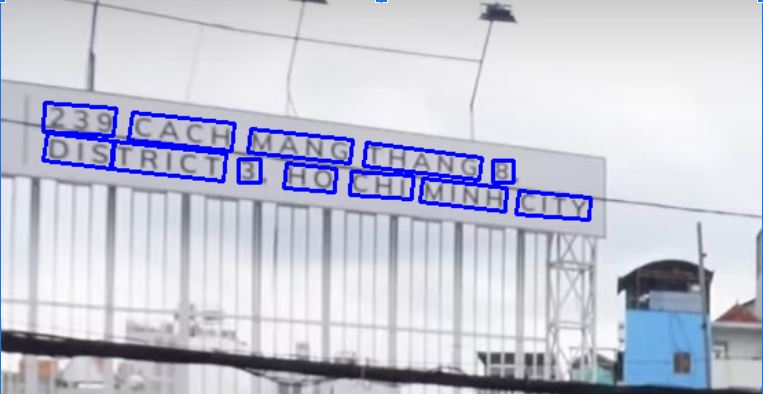
\includegraphics[width=0.9\textwidth]{mep_img/Capture2.JPG}
\caption{Bài toán phát hiện văn bản trở thành bài toán phát hiện vật thể.}\label{fig_2.4}
\end{figure}


\item Phân đoạn vật thể: Bài toán phân đoạn vật thể là một bài toán phân loại từng pixel
trên ảnh thuộc về những lớp nào (minh họa hình ~\ref{fig_2.5}). Để áp dụng phương pháp này vào quá trình phát
hiện văn bản, ta có thể sử dụng một mô hình phân loại pixel để phân loại phần pixel
nào trên ảnh là văn bản. Có thể kể đến U-Nets\cite{fink2018baseline} - một mô hình phân đoạn
ảnh nổi tiếng làm tiền đề cho những mô hình phân đoạn ảnh sau này cho tác vụ
phân đoạn văn bản trên ảnh như CRAFT\cite{baek2019character}.

\begin{figure}
\centering
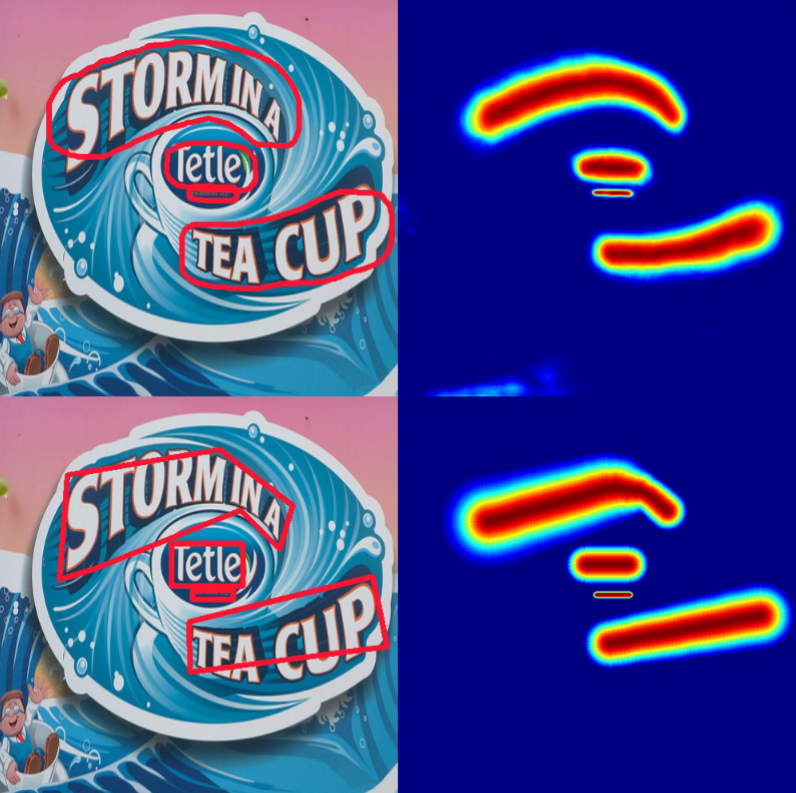
\includegraphics[width=0.9\textwidth]{mep_img/tutorial_segmentation.png}
\caption{Bài toán phát hiện văn bản trở thành bài toán phân đoạn vật thể trên từng pixel \cite{ocr_struct}.}\label{fig_2.5}
\end{figure}

\end{itemize}

Baek và các cộng sự \cite{baek2019character} đã đề xuất một phương pháp phát hiện văn bản có tên là CRAFT -
Character-Region Awareness For Text detection. Đây là một mô hình khá nổi tiếng và hoạt
động khá tốt trên những tập dữ liệu đa ngôn ngữ. CRAFT thực hiện công việc xác định vùng
của các ký tự đồng thời xác định vùng nối của các ký tự gần nhau. Mặc dù có hiệu suất tốt
nhưng CRAFT lại thực sự kém hiệu quả với những văn bản ở dạng đa hướng vì cấu trúc
của nó khá là khác so với dữ liệu hình ảnh được huấn luyện. Quá trình training mô hình này
được thể hiện như sau:
\begin{itemize}
    \item Đầu tiên, ta phải tạo ra được Synthetic Image, là tập dữ liệu hình ảnh có chưa
những đoạn văn bản được đánh nhãn ở cấp độ ký tự. Ngoài ra, ta sử dụng hai đại
lượng để tính toán độ chính xác của mô hình phát hiện văn bản là region score (có
thể coi đại lượng này giống như IOU - đại lượng đo độ trùng lặp của bounding box
được dự đoán và bounding box nhãn của hình ảnh) và affinity score. Để giải thích về
affinity score, ta có thể giả sử ta có hai ký tự liền kề được đánh nhãn bằng 2
bounding box hình chữ nhật nằm cạnh nhau. Với mỗi hình chữ nhật ta vẽ hai đường chéo, từ hai đường chéo này ta xác định được 2 tam giác trên và dưới. Ta thực hiện
công việc nối tâm của mỗi tam giác lại với nhau tạo thành một tứ giác mới được gọi
là affinity box. Và affinity score được tính toán bởi độ bao phủ hay độ trùng lặp của
các affinity box được mô hình dự đoán ra so với cái affinity box nhãn gốc. Affinity
score được dùng để xác định mỗi quan hệ của 2 từ liền kề nhau xem chúng có phải
cùng thuộc một từ hay không. Quá trình tính toán region score và affinity score được thể hiện ở hình ~\ref{fig_2.6}.

\begin{figure}
\centering
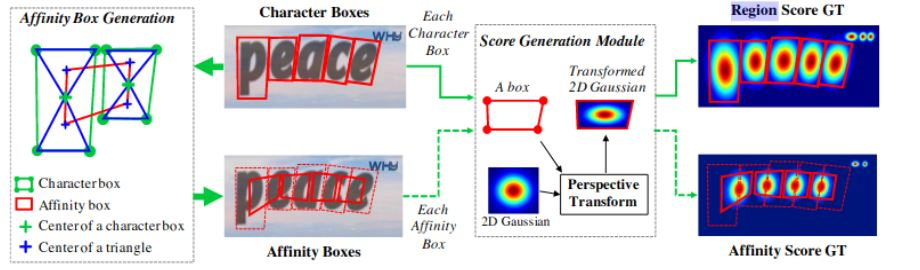
\includegraphics[width=0.9\textwidth]{mep_img/Capture3.JPG}
\caption{Quá trình tính toán của region score và affinity score \cite{baek2019character}. }\label{fig_2.6}
\end{figure}

\item Ngoài Synthetic Image, ta còn có một bộ dữ liệu ảnh thực được đánh nhãn ở cấp độ
từ được gọi là tập dữ liệu thực tế. CRAFT\cite{baek2019character} sẽ được huấn luyện bằng phương pháp
Weakly-Supervised learning \cite{zhou2018brief}. Trong mỗi lần lặp trong quá trình học (hay còn gọi là
mỗi epoch), mô hình sẽ được đem đi dự đoán trên tập dữ thực tế ở cấp độ từ thành
các bounding box ở cấp độ ký tự. Các đại lượng như Region Score và Affinity Score
đã được giới thiệu ở trên sẽ được tính toán và sử dụng như hàm \textit{loss} để cập nhật lại
trọng số của mô hình bằng Gradient Descent.
\item Kiến trúc chính của CRAFT bao gồm một mạng BackBone dùng để trích xuất những
đặc trưng có trong ảnh như là Resnet18, VGG16 vì chúng đơn giản, không tốn quá
nhiều chi phi và thời gian tính toán. Những đặc trưng này chính là những màu sắc,
cấu trúc, biên cạnh có trong ảnh. Ngoài ra, CRAFT \cite{baek2019character} còn có thêm một số cấu trúc
skip-connection giúp cho mô hình giữ được nhiều thông tin sau khi đi qua nhiều bộ
lọc tích chập và quan trọng nhất là giúp mô hình giảm thiểu tình trạng gradient
vanishing. Bên cạnh đó, vì CRAFT là một trong những phương pháp phân đoạn văn
bản trên ảnh nên mô hình này ít nhiều gì cũng bị ảnh hưởng bởi mô hình mạng
U-Nets. Điển hình ở đây là các lớp De-Convolution hay tích chập ngược và các
skip-connection khiến cho kiến trúc của CRAFT có hình chữ U (giống U-Nets) với các
lớp Convolution đi xuống và De-Convolution đi lên. Kiến trúc của CRAFT \cite{baek2019character} được mô tả kiến trúc ở hình ~\ref{fig_2.7}

\begin{figure}
\centering
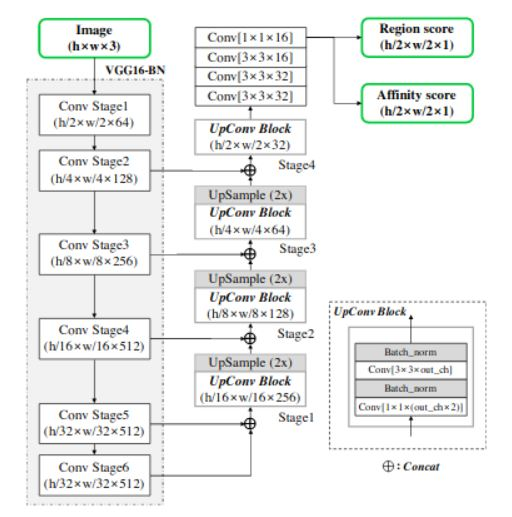
\includegraphics[width=0.9\textwidth]{mep_img/Capture4.JPG}
\caption{Kiến trúc giống mạng U-Nets của mô hình CRAFT \cite{baek2019character}. }\label{fig_2.7}
\end{figure}

\end{itemize}
Ngoài CRAFT ra, CTPN \cite{tian2016detecting} cũng là một mô hình khá nổi tiếng được sử dụng nhiều trong tác vụ phát hiện văn bản. Mô hình này được phân loại vào nhóm phương pháp phát hiện vật thể (vật thể ở đây chính là văn bản) trên ảnh. Giống như CRAFT, mô hình này cũng sử dụng VGG16 làm một mạng con BackBone trong tác vụ trích xuất đặc trưng trên ảnh. Ngoài ra, Sliding-window - một kỹ thuật trong phát hiện vật thể trên ảnh bằng những bộ lọc tích chập, cũng được sử dụng để tìm vùng nào trên ảnh có thể chứa văn bản. Sau đó, các đặc trưng sẽ được đưa qua một mô hình RNN đơn giản và một lớp fully-connected cuối cùng. Kết quả của mô hình sẽ trả về xác suất có văn bản trong một vùng, tọa độ của bounding box chứa vùng đó. 
\subsection{Text Recognition}
Phần kế tiếp của một mô hình OCR sau khi phát hiện được vị trí của văn bản trong ảnh
chính là nhận diện xem phần văn bản đó là gì, chúng đại diện và thể hiện cho điều gì. Một
số mô hình đạt được hiệu suất tốt trong bài toán này có thể kể đến như Deep Text
Recognition BenchMark \cite{baek2019wrong} và VietOCR \cite{VietOCR}.

Deep Text Recognition BenchMark là một mô hình nhận diện ký tự được đề xuất vào năm 2019. Quá trình hoạt động của mô hình được mô tả
trong hình~\ref{fig_2.8}.

\begin{figure}
\centering
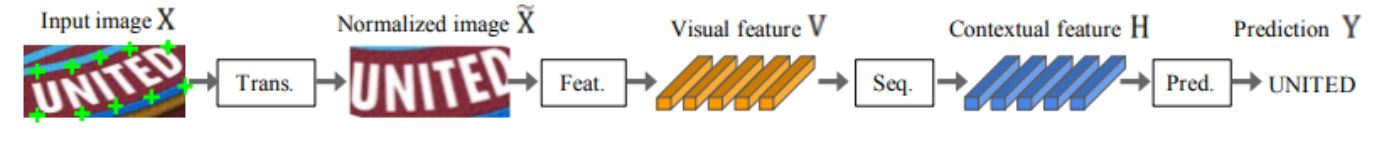
\includegraphics[width=0.9\textwidth]{mep_img/Capture5.JPG}
\caption{Mô hình Deep Text Recognition \cite{baek2019wrong}. }\label{fig_2.8}
\end{figure}

Văn bản có trong hình ảnh (nằm trong 1 bounding box) có thể có nhiều hướng khác nhau
ảnh hưởng đến quá trình dự đoán của mô hình. Nên việc đầu tiên cần làm chính là khử độ
nghiêng, đưa văn bản về 1 hướng duy nhất (các tác giả gọi bước này là chuẩn hóa hình ảnh
ban đầu X thành hình ảnh chuẩn hóa X’). Tiếp theo, hình ảnh đã được chuẩn hóa sẽ được
đưa vào một mô hình mạng BackBone đơn giản để trích xuất đặc trưng như đã nói ở phần
CRAFT, những mạng này có thể là VGG16 hoặc Resnet. Sau đó những đặc trưng được
trích xuất ra sẽ được đưa vào một mô hình đặc biệt được gọi là Sequence Model để huấn
luyện và sẽ giữ lại những đặc trưng liên quan đến ngữ cảnh, từ đó những đặc trưng này sẽ
làm đầu vào cho quá trình nhận diện văn bản.

Mặc dù, mô hình trên được đánh giá là hoạt động tốt trên bộ dữ liệu văn bản tiếng Anh, tuy
nhiên khi sử dụng trên bộ dữ liệu bằng tiếng Việt thì mô hình hoạt động kém hiệu quả. Bởi
lẽ ngôn ngữ Việt có những đặc trưng rất riêng mà tiếng Anh không có. Lấy ví dụ cùng là chữ
A trong tiếng anh, nhưng sang tiếng Việt lại có rất nhiều sắc thái và ngữ nghĩa khác nhau
như: Ă, Á, À,... .

VietOCR \cite{VietOCR} là một mô hình nhận dạng văn bản, chữ viết dành riêng cho người Việt có mã
nguồn mở (miễn phí), có thể dùng với cả chữ viết tay và chữ in. Mô hình này đã kết hợp các
mô hình Deep Learning NLP vào hệ thống Text Recognition làm tăng độ chính xác khi nhận
diện văn bản dựa theo ngữ cảnh. VietOCR cung cấp cho người dùng lựa chọn giữa 2 kiểu
model ngôn ngữ tương ứng với hai kiểu cài đặt Attention OCR và Transformer OCR.

Attention OCR \cite{VietOCR} là sự kết hợp của CNN và Attention Seq2Seq \cite{galassi2020attention}. Đầu vào của mô hình là một
bức ảnh được đưa vào mô hình CNN, sẽ cho một feature maps có kích thước
\textbf{channel*height*width}, và được đưa vào mô hình LSTM để dự đoán. Tuy nhiên, mô hình
LSTM chỉ nhận đầu vào có kích thước là một ma trận đặc trưng 2 chiều. Để giải quyết vấn
đề này, ta thực hiện công việc gộp 2 chiều height và width của ma trận lại làm một, tạo
thành một ma trận mới có kích thước \textbf{channel*(height*width)}. Feature maps lúc này sẽ có
kích thước phù hợp với yêu cầu của mô hình LSTM - đây là một mô hình khá nổi tiếng trong
lĩnh vực Natural Language Processing, mô hình này có khả năng chọn ra những từ nào
trong văn bản là quan trọng, và những đặc trưng của từ đó sẽ trở thành đầu vào cho những
từ tiếp theo trong câu.

Transformer \cite{gillioz2020overview} có thể thay thế cho LSTM để đưa ra dự đoán cho các từ được phát hiện trong
ảnh cũng như các từ có thể xuất hiện tiếp theo. Thay vì xử lý câu một cách tuần tự như
những mô hình ngôn ngữ khác, Transformer thực hiện việc xử lý song song các từ trong
cùng một câu để giảm thời gian xử lý đáng kể. Mô hình này sử dụng cơ chế self-attention,
không giống như kiến trúc hồi quy của RNNs với 6 bộ encoder và 6 bộ decoder. Mỗi
encoder và decoder chứa hai lớp: Self-attention và mạng truyền thẳng (FNN). Self-Attention
giúp cho Transformers có thể hiểu được sự liên quan giữa các từ trong một câu, kể cả khi
chúng có khoảng cách xa. Tuy nhiên một lớp attention được chèn vào giữa các decoder để
mô hình vẫn giữ đươc những đặc trưng và sự liên kết của những từ trước đó.

\subsection{Post-OCR}

Công đoạn cuối cùng của một hệ thống OCR hoàn chỉnh đó chính là Post-OCR, hay hậu xử
lý OCR. Tùy thuộc vào bài toán và từng trường hợp cụ thể gặp phải mà sau khi OCR ta có
những bước xử lý khác nhau. Ví dụ trong bài toán OCR dữ liệu từ sách thành dữ liệu PDF
trên máy. Ta cần một phương pháp hậu xử lý đảm bảo tất cả dữ liệu văn bản được trọn vẹn,
không thiếu sót cũng như không sai chính tả thì thường bên sử dụng hệ thống sẽ chọn
những phương pháp thủ công do con người đích thân chữa lỗi (Survey of post-ocr processing approaches \cite{nguyen2021survey}).

Bên cạnh đó, với sự phát triển của mảng NLP trong thời gian gần đây, việc càng có nhiều
mô hình ứng dụng các mô hình ngôn ngữ vào quá trình hậu xử lý đã không còn quá xa lạ.
Chúng đem lại những kết quả rất tốt, bám sát theo yêu cầu xử lý văn bản mà người dùng
đặt ra. Trong nội dung của khóa luận này, chúng tôi sẽ giới thiệu một số mô hình cũng như
thuật toán có ích trong việc giúp giải quyết bài toán hậu xử lý sau khi OCR đơn thuốc.

\section{Regular Expression}

\textbf{Regular Expression}, hay còn gọi là RegEx, là một công cụ mạnh mẽ để xử lý các loại văn bản. Trong bài toán trích xuất thông tin, đầu vào của ta thường là một tập các thông tin hỗn độn, và ta có nhu cầu chỉ trích ra một phần thông tin có giá trị trong số đó. Nếu như cấu trúc thông tin của input này là tương đối rõ ràng, chúng ta hoàn toàn có thể xây dựng một tập các heuristic rules, hay còn gọi là mẫu (pattern), nhằm lấy được đúng thứ mình cần. Đối với trường hợp này, RegEx là một công cụ mạnh mẽ và tương đối hiệu quả về cả độ chính xác cũng như chi phí thời gian.

Ví dụ, ta có chuỗi "STT: 1 Họ và tên: Nguyễn Văn A", ta có thể dùng luật để tách được số thứ tự, họ tên và giới tính trong chuỗi này theo mẫu như sau: \textbf{"^STT: (.*?) Họ và tên: (.*?) Giới tính: (.*?)$\$$"}. Trong đó, kí tự đầu tiên \textbf{"\^"} đại diện cho đầu dòng văn bản, và\textbf{"\$"} là cuối dòng văn bản. Các cụm ngoặc đơn đại diện cho nội dung mình muốn lấy, bên trong là ".*?" đại diện cho một tập các kí tự bất kì. Hình ~\ref{regex_1} chỉ ra phần giải thích chi tiết cho mẫu này, được chạy thử ở trang \textit{regex101} \footnote{https://regex101.com/r/G9VcLD/1}.

\begin{figure}
\centering
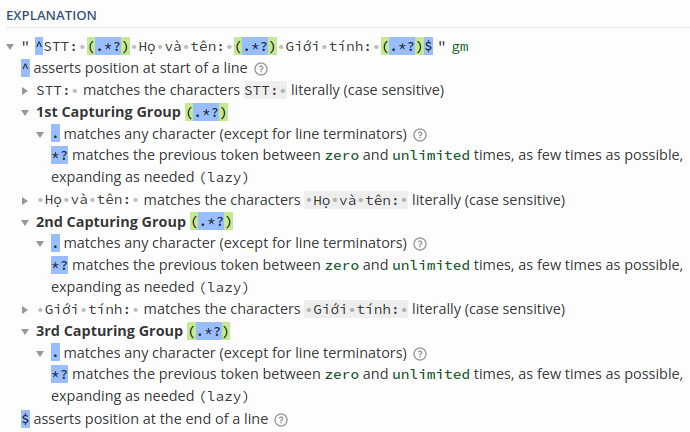
\includegraphics[width=0.8\textwidth]{mep_img/regex_1.png}
\caption{Giải thích chi tiết cho regex trích xuất thông tin người dùng.}\label{regex_1}
\end{figure}

\begin{figure}
\centering
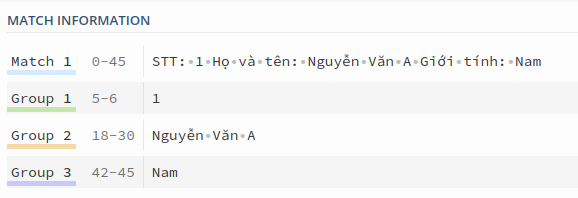
\includegraphics[width=0.8\textwidth]{mep_img/regex_2.png}
\caption{Kết quả thực tế cho RegEx trích xuất thông tin người dùng, bao gồm 3 phần riêng biệt là 3 thông tin mà ta muốn lấy.}\label{regex_2}
\end{figure}

Kết quả của câu RegEx phía trên khi chạy trên dữ liệu ví dụ cho ra được kết quả như trong hình ~\ref{regex_2}. Như vậy, chúng ta hoàn toàn có thể dùng RegEx để ứng dụng vào bài toán trích xuất tên thuốc để đảm bảo tối ưu mô hình. 

\section{TCN}

Để xác định chuỗi văn bản là thuốc nào trong cơ sở dữ liệu, bài toán Text Classification cần được chúng tôi xem xét. Các mô hình dựa trên CNN thường được áp dụng do kết quả thực thi tốt trên các văn bản đơn giản. Tuy nhiên, khi văn bản nhập nhằng hay chứa nhiều đặc trưng khác nhau thì chúng không còn xử lý tốt nữa. Để khắc phục, các mô hình thuộc nhóm \textit{recurrent} (RNN) được đề xuất như LSTM hay GRU. Chúng có thể học được đặc trưng chuỗi liền mạch giống như cách bộ não con người xử lý (theo kiểu trình tự). Từ đó các mô hình này có thể hiểu được thông tin ngữ cảnh dùng trong mỗi văn bản.

Một điểm yếu của các thuật toán dựa trên RNN là chi phí tính toán cao hơn nhiều so với CNN. Shaojie Bai và các cộng sự \cite{bai2018empirical} đã giới thiệu một kỹ thuật mới là temporal convolutional network (TCN). Nó là một phiên bản nhỏ gọn của CNN. Cụ thể, nó dựa trên mạng tích chập giãn nở (dilated convolutions). Các mạng tích chập giãn nở này cho phép TCN học được các đặc trưng trong quá khứ (không bao gồm các thông tin ở tương lai). Mỗi output $y_t$ sẽ dựa trên mỗi chuỗi các input $x$ được lọc (filter size) trên \verb|{0, 1, …, t-1, t}|. Bằng cách chỉnh các tham số \verb|d| (dilation factor) và \verb|k| (filter size), ta có thể quyết định được độ sâu cần thiết trong quá khứ mà mô hình muốn học. 

Với tính giãn nở đó, cách hoạt động của TCN mang lại tính đột phá và có tính \textit{recurrent} tương tự RNN. Điều đó giúp đảm bảo cả về hiệu năng, cũng như cho ra kết quả tốt so với các mô hình thuộc họ RNN. Hình ~\ref{tcn} minh họa kiến trúc của mô hình TCN.

\begin{figure}
\centering
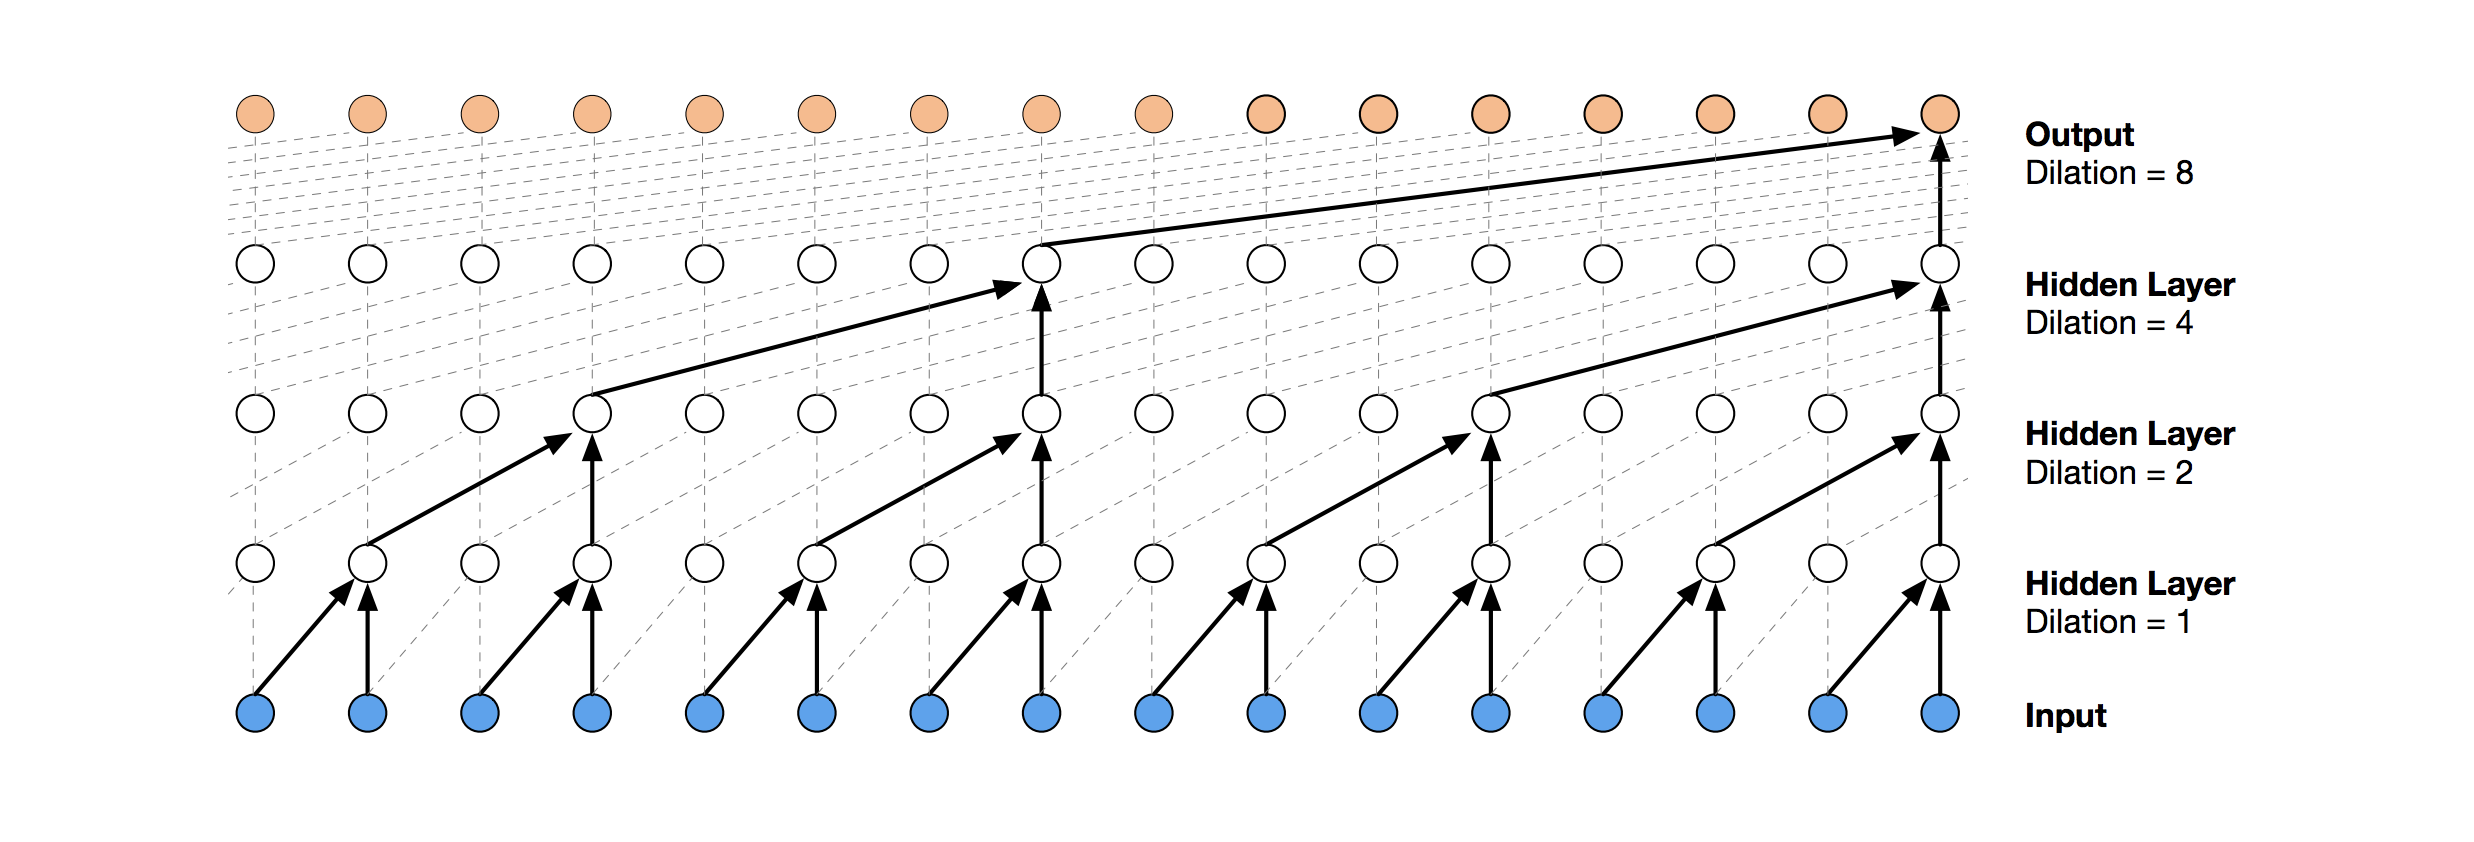
\includegraphics[width=1.0\textwidth]{mep_img/TCN.png}
\caption{Cách hoạt động của kiến trúc mạng TCN, giúp nó có tính liền mạch giống như các mô hình RNN nhưng vẫn đảm bảo xử lý trong thời gian ngắn.}\label{tcn}

\end{figure}

Trong bài toán nhận dạng tên thuốc, ta cũng cần phân biệt tên thuốc, là một hay một số từ có thể mang đặc trưng riêng trong lĩnh vực y học, khác với các văn bản thông thường khác. Như vậy chúng tôi hoàn toàn có thể ứng dụng TCN trong bài toán nhận dạng tên thuốc, và sẽ tiếp tục được đề cập đến ở phần phương pháp đề xuất.

% \section{Dataset}

% Một trong những yếu tố có thể được coi là quan trọng nhất giúp xây dựng một hệ thống
% OCR đạt hiệu suất tốt chính là tập dữ liệu. Trong phần này, chúng tôi sẽ giới thiệu một số
% tập dữ liệu được sử dụng trong tác vụ huấn luyện cũng như đánh giá một mô hình OCR.
% \begin{itemize}
%     \item \textbf{ICDAR 2013}: Đây là bộ dữ liệu có chứa 229 hình ảnh được sử dụng cho quá trình
% training mô hình và 233 hình ảnh được dùng cho quá trình đánh giá thời gian và độ
% chính xác. Ngoài ra, những phần văn bản có trong ảnh được đánh nhãn ở cấp độ từ
% và tập dữ liệu này còn được gọi là tập dữ liệu tiêu chuẩn để đánh giá các mô hình
% OCR.
% \item \textbf{ICDAR 2015}: Cũng gần giống như tập dữ liệu ICDAR 2013, tập dữ liệu này bao gồm
% 1000 hình ảnh được dùng cho quá trình training và 500 hình ảnh được dùng cho quá
% trình đánh giá. Bộ dữ liệu này được dùng cho rất nhiều cuộc thi về OCR.
% \item \textbf{CTW}: Tập dữ liệu bao gồm 32285 hình ảnh với độ phân giải cao và bao gồm hơn 1
% triệu ký tự, từ,... . Phần văn bản trong ảnh được đánh nhãn ở cấp độ ký tự.
% \end{itemize}
% Mặc dù trên thực tế đã có rất nhiều tập dữ liệu khác nhau với kích thước vô cùng lớn và
% hình ảnh đa dạng, tuy nhiên với một mô hình phục vụ cho bài toán OCR trên đơn thuốc của
% chúng tôi thì những tập dữ liệu trên là chưa đủ. Không giống như những tập dữ liệu kể trên,
% với hình ảnh đơn thuốc, vùng chữ thường có khoảng cách rất gần nhau và phông chữ đôi
% khi không được đồng đều ảnh hưởng đến quá trình OCR và Post-OCR. Vì thế, chúng tôi đã
% thực hiện công việc thu thập và xây dựng một bộ data bám sát vào bài toán và mô hình của
% chúng tôi. Bộ dữ liệu đó có tên là \codeword{Prescription Dataset}. Chúng tôi sẽ giới thiệu chi tiết hơn
% về tập dữ liệu này trong phần sau.